\section{Testen}\label{section:konzeption:testen}

% \begin{note}
%     \textbf{Notizen:}
%     \begin{itemize}
%         \item Erwähnung von \autoref{requirement:Testen}
%         \item Beschreibung der CrossLab-Services + Klassendiagramm
%         \item Beschreibung der Einbindung in die betrachtete Experimentkonfiguration
%     \end{itemize}
% \end{note}

Nach \autoref{requirement:Testen} soll ein CrossLab-Service für die Erstellung und Ausführung von Testfällen innerhalb eines Experiments entwickelt werden. Dabei soll nach Unteranforderung (a) der Producer in der Lage sein, Funktionen zur Verwendung in Testfällen bereitzustellen. Unteranforderung (b) verlangt, dass diese Funktionen vom Consumer ausgeführt werden können. Die Erstellung von Testfällen soll laut Unteranforderung (c) während der Konfiguration eines Experiments erfolgen können. Außerdem soll der entwickelte CrossLab-Service nach Unteranforderung (d) von der IDE zur Ausführung von Testfällen innerhalb eines Experiment verwendet werden. Dementsprechend wird im Folgenden der \textit{Testing Service} vorgestellt.

\autoref{figure:klassendiagramm-testing-service} zeigt ein Klassendiagramm für den Testing Service. Der Testing Service Producer ermöglicht es Laborgeräten Funktionen für die Erstellung von Testfällen bereitzustellen. Diese müssen über die Funktion \texttt{registerFunction()} registriert werden. Dabei werden mindestens der Name der Funktion und deren Implementierung benötigt. Zusätzlich könnte man die Angabe von Schemata für die Argumente und den Rückgabewert der Funktion verlangen. Diese ermöglichen die Validierung der Eingaben und Ausgaben der Funktion. Der Testing Service Consumer erlaubt das Hinzufügen von Testfällen über die Funktion \texttt{addTest()}. Tests bestehen dabei aus einem Namen, einer Liste an Funktionen und ggf. eine Liste von weiteren Tests. Funktionen werden durch ihren Namen, den Kennzeichner des bereitstellenden Testing Service Producer und ihre Argumente beschrieben. Zusätzlich kann ein erwarteter Rückgabewert angegeben werden. Dieser wird während dem Testen mit dem tatsächlichen Rückgabewert verglichen. Sollten die Werte dabei unterschiedlich sein, schlägt der Testfall fehl. Angenommen, das Experiment beinhaltet einen Microcontroller, der das Setzen und Auslesen seiner Pins über entsprechende Funktionen ermöglicht. Durch die Angabe von erwarteten Rückgabewerten kann beim Auslesen der Pins sichergestellt werden, dass der zu diesem Zeitpunkt erwartete Wert vorliegt. Die weiteren Testfälle werden nach den Funktionen in der angegebenen Reihenfolge ausgeführt. Der Testing Service Consumer kann das Testen über die Funktion \texttt{startTesting()} beginnen. Dadurch wird ein entsprechendes \texttt{StartTesting}-Event bei den Test Service Producern ausgelöst. Über entsprechende Event Handler können Vorbereitungen für die Ausführung der Testfälle getroffen werden, bevor eine Antwort an den Testing Service Consumer gesendet wird. Sobald alle Testing Service Producer eine Antwort gesendet haben, kann der Testing Service Consumer mithilfe der Funktion \texttt{runTest()} Testfälle ausführen. Dafür werden für jeden Testfall zunächst dessen Funktionen der Reihe nach aufgerufen und danach die weiteren enthaltenen Testfälle in der angegebenen Reihenfolge ausgeführt. Nachdem alle ausgewählten Testfälle ausgeführt wurden, kann die Operation \texttt{endTesting()} des Testing Service Consumer genutzt werden, um das Testen zu beenden. Hierbei wird wieder ein entsprechendes \texttt{EndTesting}-Event von den Testing Service Producern ausgelöst, welches über Event Handler genutzt werden kann, um den Normalzustand wiederherzustellen.

\begin{figure}[tbp]
    \centering
    \begin{tikzpicture}
        \begin{class}[text width=6cm]{TestingServiceProducer}{0,0}
            \operation{+ registerFunction()}
            \operation{+ onStartTesting()}
            \operation{+ onEndTesting()}
            \operation{+ onFunctionCall()}
        \end{class}
        \begin{class}[text width=6cm]{TestingServiceConsumer}{7,0}
            \operation{+ addTest()}
            \operation{+ runTest()}
            \operation{+ startTesting()}
            \operation{+ endTesting()}
        \end{class}
    \end{tikzpicture}
    \caption{Klassendiagramm Testing Service}
    \label{figure:klassendiagramm-testing-service}
\end{figure}

Die Einbindung des Testing Service in die betrachtete Experimentkonfiguration kann z.B. über das Hinzufügen eines Testing Service Consumer bei der IDE und eines Testing Service Producer bei der Steuereinheit erfolgen. Für ein konkreteres Beispiel wird ein Microcontroller als Steuereinheit angenommen. Dieser könnte das Setzen und Auslesen der Werte seiner Pins als Funktionen für Testfälle anbieten. Diese können für die Erstellung von Testfällen genutzt werden, die während dem laufenden Experiment von der IDE ausgeführt werden können.

\begin{figure}[htbp]
    \centering
    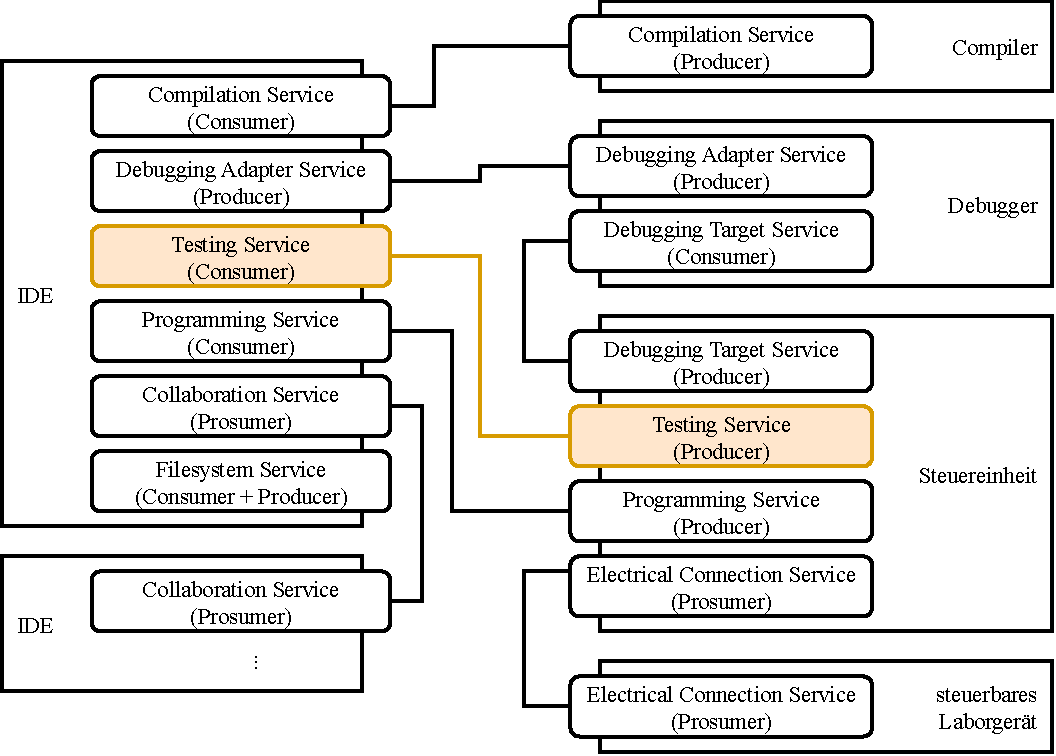
\includegraphics[width=\textwidth]{diagrams/experimentkonfigurationen/Experimentkonfiguration-05.drawio.pdf}
    \caption{Experimentkonfiguration}
    \label{figure:experimentkonfiguration:testen}
\end{figure}